\documentclass[sigconf,anonymous,review]{acmart}

%%
%% Packages and Configuration
%%
\usepackage{booktabs}
\usepackage{amsmath}
\usepackage{amsfonts}
\usepackage{subcaption}
\usepackage{tikz}
\usetikzlibrary{shapes,arrows.meta,positioning,fit,backgrounds,calc}

%%
%% Rights management information.
%%
\setcopyright{none}
\acmConference[Preprint]{Review Manuscript}{October 2026}{Changa, India}
\acmYear{2026}
\acmDOI{}
\acmISBN{}

%%
%% Document starts
%%
\begin{document}

\title{AI Firewall: A Shared, Risk-Based Authorization Gateway with Exact-Action Human Approval Binding for Autonomous AI Agents}

%%
%% Double-Blind Anonymization: Author block is suppressed by the [anonymous] class option.
%%
\author{Anonymous Author(s)}
\affiliation{
  \institution{Anonymous Institution}
  \country{}
}
\email{}

%%
%% Abstract
%%
\begin{abstract}
As Large Language Model (LLM) agents are granted autonomous access to external environments via tool execution APIs and standardized protocols like the Model Context Protocol (MCP), they become susceptible to indirect prompt injection, tool poisoning, and unauthorized capability execution. Existing defenses rely heavily on model alignment, prompt filtering, or custom language interpreters; however, these techniques either fail against adaptive attacks or lack binding authorization mechanisms when human-in-the-loop oversight is required. 

This paper presents \textbf{AI Firewall}, a shared, risk-based authorization gateway that mediates tool invocations across heterogeneous agent adapters prior to downstream execution. AI Firewall enforces a tripartite security protocol: (1) deterministic transformation of heterogeneous tool proposals into canonical action identities using RFC 8785 JSON Canonicalization and SHA-256 digests; (2) declarative policy evaluation that computes risk scores and mandates cryptographic Ed25519 approval envelopes bound to the exact canonical action digest; and (3) transactional lifecycle fencing on SQLite with monotonic worker epochs that prevents approval replay, parameter tampering, and post-timeout execution races.

We evaluate AI Firewall through an empirical evaluation across a formal 46-scenario security benchmark (31 consequential attacks and 15 legitimate tasks), supported by a comprehensive 107-test regression suite. In the evaluated benchmark suite, AI Firewall successfully blocked 31 of 31 consequential attacks (100.0\% observed, Clopper--Pearson 95\% exact binomial confidence interval [88.8\%, 100.0\%]) while executing 15 of 15 legitimate tasks without false denials (100.0\% observed utility, 95\% CI [78.2\%, 100.0\%]). Under a thread-bounded connection registry optimization, median authorization overhead is reduced by \textbf{81.29\%} (from 3.0153\,ms to 0.5643\,ms), with P99 tail latency dropping by \textbf{95.97\%} (from 24.0348\,ms to 0.9679\,ms) and batch throughput scaling to \textbf{1,716.4 operations per second}. We verify protocol interoperability across MCP stdio child processes and simulated LangGraph-style workflows, and formalize the downstream execution boundary where tool idempotency is required to guarantee end-to-end execution safety upon network timeouts.
\end{abstract}

%%
%% Keywords
%%
\keywords{AI Agent Security, Runtime Authorization, Tool Use, Prompt Injection, Model Context Protocol, Cryptographic Approval Envelopes, Fencing Tokens}

\maketitle

%%
%% Section 1: Introduction
%%
\section{Introduction}

Autonomous AI agents powered by Large Language Models (LLMs) are transitioning from isolated chat interfaces into proactive systems that invoke external APIs, query relational databases, alter file systems, and execute code on behalf of human users~\cite{greshake2023not, debenedetti2024agentdojo}. To facilitate tool interoperability, industry architectures have rapidly converged on shared protocols such as Anthropic's Model Context Protocol (MCP)~\cite{mcp2024spec} and agent orchestration frameworks such as LangChain and LangGraph.

However, giving LLMs the autonomy to execute external tools introduces severe security risks. When an agent processes untrusted external data---such as web pages, email bodies, or database query results---an adversary can embed adversarial instructions known as \emph{indirect prompt injection} (IPI)~\cite{greshake2023not}. These injected instructions hijack the model's reasoning loop, causing it to invoke consequential tools without user knowledge, exfiltrate confidential data, or destroy critical infrastructure.

Recent security literature has proposed diverse countermeasures. \emph{DataSentinel}~\cite{liu2025datasentinel} explores game-theoretic prompt filtering; however, purely text-based classifiers suffer from false positives and remain vulnerable to adaptive prompt evasions. \emph{IsolateGPT}~\cite{wu2025isolategpt} isolates application execution contexts, and \emph{CaMeL}~\cite{debenedetti2025camel} enforces capability-based information flow tracking within a custom Python interpreter. Similarly, \emph{Progent}~\cite{shi2025progent} uses domain-specific languages and SMT solvers to enforce monotonic privilege narrowing. 

Despite these advancements, an architectural vulnerability remains at the boundary between agent decision-making and external tool dispatch: \textbf{the absence of a shared, protocol-agnostic authorization gateway that cryptographically binds human approval to the exact tool call being executed.} When current frameworks implement human-in-the-loop (HITL) checkpoints:
\begin{enumerate}
    \item \textbf{Approval Substitution \& Tampering:} Approvals are typically granted in natural language or against coarse user prompts rather than the exact serialized parameters sent over the network wire. An attacker can manipulate arguments after an approval is granted or substitute a destructive action for a benign one.
    \item \textbf{Replay \& Concurrency Races:} Frameworks lack transactional lifecycle management to ensure that an approval envelope is redeemed strictly once. In concurrent or distributed agent worker environments, network timeouts or retries can cause duplicate executions of non-idempotent actions.
    \item \textbf{Cross-Adapter Inconsistencies:} Different frameworks (e.g., LangChain vs. MCP) employ disparate parameter naming conventions, casing, and serialization formats, making centralized policy auditing impossible.
\end{enumerate}

\subsection{Our Contributions}
In this paper, we introduce \textbf{AI Firewall}, an independent, risk-based authorization gateway designed to sit between AI agent frameworks and downstream tool servers. Our primary contributions are:
\begin{enumerate}
    \item \textbf{Exact-Action Canonicalization \& Cryptographic Envelope Binding:} We implement an RFC 8785 JSON Canonicalization Scheme (JCS) hasher~\cite{rfc8785} that maps heterogeneous tool proposals into unique SHA-256 digests. Human approvals are signed using Ed25519 cryptographic envelopes~\cite{rfc8032} that bind directly to this digest, eliminating parameter tampering, substitution, and authentication-downgrade attacks.
    \item \textbf{Transactional State Machine with Monotonic Fencing:} We design an ACID-compliant authorization lifecycle on SQLite. By combining single-use nonces, \texttt{BEGIN EXCLUSIVE TRANSACTION} reservation semantics, and monotonic dispatch epoch counters (\texttt{dispatch\_epoch}), the gateway ensures single-use redemption and fences off stale or crashed workers.
    \item \textbf{Empirical Performance Profiling \& Optimization:} We identify that persistence connection setup accounts for over 98\% of gateway overhead in naive on-demand implementations. We design and validate a manager-owned thread connection registry that reduces median authorization latency from \textbf{3.0153\,ms to 0.5643\,ms (81.29\% reduction)}, scaling single-core throughput to \textbf{1,716.4\,ops/sec}.
    \item \textbf{Empirical Evaluation \& Multi-Adapter Verification:} We evaluate AI Firewall across a 46-scenario security benchmark and a 107-test unit regression suite, evaluating crash recovery across an 8-scenario failure matrix, real OS child-process MCP stdio framing, and simulated LangGraph interrupt/checkpoint cycles. We establish an evidence baseline and formalize the limits of gateway fencing when downstream tools lack server-side idempotency.
\end{enumerate}

%%
%% Section 2: Related Work
%%
\section{Background and Related Work}

\begin{table*}[t]
\centering
\caption{Comparison of AI Firewall against representative AI agent defense architectures.}
\label{tab:related_work}
\small
\begin{tabular}{lllll}
\toprule
\textbf{Approach} & \textbf{Enforcement Locus} & \textbf{Policy Model} & \textbf{Human Approval Binding} & \textbf{Adapter Scope} \\
\midrule
DataSentinel~\cite{liu2025datasentinel} & Prompt Classifier & Minimax Detection & None & Unmediated Prompts \\
IsolateGPT~\cite{wu2025isolategpt}     & App Isolation Sandbox & Coarse Sandbox Rules & Unbound Natural Language & Natural Language APIs \\
CaMeL~\cite{debenedetti2025camel}         & Python Interpreter & Information Flow / Capabilities & None (Capability Rules) & In-Interpreter Values \\
Progent~\cite{shi2025progent}             & Agent Execution Loop & SMT Privilege DSL & None (Narrowing Rules) & LangChain / OpenAI SDK \\
\textbf{AI Firewall (Ours)}               & \textbf{External Gateway} & \textbf{Risk \& Epoch Rules} & \textbf{Cryptographic Ed25519 to RFC 8785 Digest} & \textbf{MCP \& LangChain} \\
\bottomrule
\end{tabular}
\end{table*}

\subsection{Prompt Injection and Agent Exploitation}
Indirect prompt injection was first systematically categorized by Greshake et al.~\cite{greshake2023not}, who demonstrated that arbitrary instructions embedded in retrieved data could commandeer an LLM's application context. Debenedetti et al.~\cite{debenedetti2024agentdojo} established \emph{AgentDojo}, a dynamic benchmark comprising 97 tasks and 629 security test cases, showing that prompt-based safeguards and commercial model alignments consistently fail against adaptive injection attacks.

\subsection{System-Level and Language-Level Defenses}
Recognizing that model-level alignment is insufficient, recent work has shifted toward system-level containment. Wu et al.~\cite{wu2025isolategpt} presented \emph{IsolateGPT}, which introduces execution isolation for LLM applications. Debenedetti et al.~\cite{debenedetti2025camel} introduced \emph{CaMeL}, which separates control and data flows by extracting application logic from user prompts and tracking capabilities within a custom Python interpreter, solving 77\% of AgentDojo tasks with provable security. Shi et al.~\cite{shi2025progent} proposed \emph{Progent}, which enforces least privilege using a policy DSL and an SMT solver to guarantee monotonic privilege narrowing across tool calls.

\subsection{Research Gap: Independent Gateway Authorization}
While CaMeL and Progent provide compelling defenses, they require either running code in a bespoke Python interpreter or deeply modifying the internal agent runtime loop. They do not address environments where tool execution occurs across distributed protocols (such as MCP over stdio or SSE), nor do they provide cryptographic verification when consequential actions mandate human sign-off. Furthermore, they do not account for concurrency races, stale worker fencing, or downstream retry semantics. AI Firewall addresses this gap by operating as an external, protocol-aware network mediator (Table~\ref{tab:related_work}).

%%
%% Section 3: Threat Model
%%
\section{Threat Model and Security Objectives}

\begin{figure}[t]
\centering
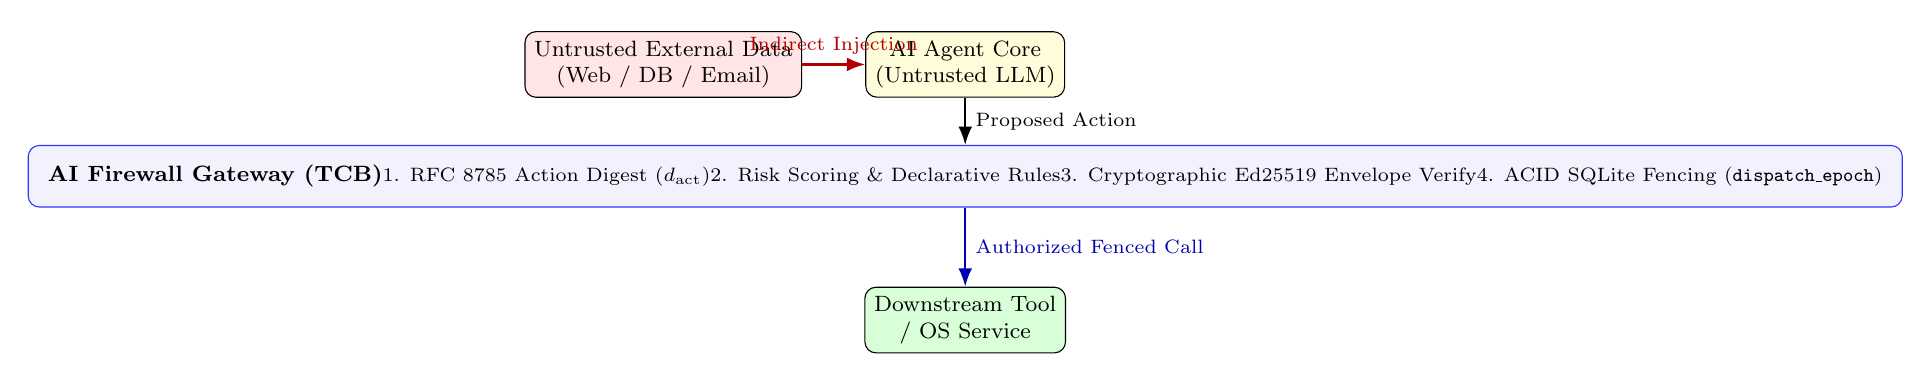
\begin{tikzpicture}[
    node distance=1.1cm and 0.8cm,
    block/.style={rectangle, draw, rounded corners, minimum height=0.7cm, minimum width=2.4cm, align=center, fill=gray!10, font=\footnotesize},
    gateway/.style={rectangle, draw=blue!80, fill=blue!5, rounded corners, inner sep=0.25cm, font=\footnotesize},
    arrow/.style={-Latex, thick}
]
\node[block, fill=red!10] (untrusted) {Untrusted External Data\\(Web / DB / Email)};
\node[block, fill=yellow!15, right=0.8cm of untrusted] (agent) {AI Agent Core\\(Untrusted LLM)};
\node[block, fill=green!15, below=2.4cm of agent] (tool) {Downstream Tool\\/ OS Service};

\draw[arrow, red!70!black] (untrusted) -- node[above, font=\scriptsize] {Indirect Injection} (agent);

\node[gateway, below=0.6cm of agent, minimum width=3.8cm] (gw) {
    \textbf{AI Firewall Gateway (TCB)}\\
    \scriptsize 1. RFC 8785 Action Digest ($d_{\text{act}}$)\\
    \scriptsize 2. Risk Scoring \& Declarative Rules\\
    \scriptsize 3. Cryptographic Ed25519 Envelope Verify\\
    \scriptsize 4. ACID SQLite Fencing (\texttt{dispatch\_epoch})
};

\draw[arrow] (agent) -- node[right, font=\scriptsize] {Proposed Action} (gw);
\draw[arrow, blue!70!black] (gw) -- node[right, font=\scriptsize] {Authorized Fenced Call} (tool);

\end{tikzpicture}
\caption{Threat model and trust boundary enforced by AI Firewall.}
\label{fig:threat_model}
\end{figure}

\subsection{Assets and Adversary Capabilities}
We consider an environment where an AI agent interacts with external resources (filesystems, databases, APIs) via tools (Figure~\ref{fig:threat_model}). 
\begin{itemize}
    \item \textbf{Adversary Capabilities:} The adversary can inject arbitrary natural language into any untrusted data source retrieved by the agent. The adversary can influence tool call parameters, attempt parameter tampering between human approval and execution, replay intercepted approvals, and manipulate concurrency timing.
    \item \textbf{Untrusted Components:} The LLM reasoning core, prompt context, and agent planning logic are untrusted.
    \item \textbf{Trusted Computing Base (TCB):} The AI Firewall gateway, its local SQLite database, the human reviewer's private key, and the gateway's cryptographic key registry are trusted.
\end{itemize}

\subsection{Security Objectives}
\begin{enumerate}
    \item \textbf{Mandatory Interception \& Policy Enforcement:} No tool proposal may execute without passing declarative policy evaluation. Explicit \texttt{DENY} rules take precedence over \texttt{ALLOW}.
    \item \textbf{Exact-Action Approval Binding:} An approval granted for action proposal $A$ cannot be redeemed to execute action proposal $A' \neq A$. Any alteration to tool names, resource URIs, or arguments must invalidate the approval.
    \item \textbf{Single-Use Replay Resistance:} An approval envelope cannot be redeemed more than once, even across concurrent worker threads or restarted processes.
    \item \textbf{Monotonic Dispatch Fencing:} Stale workers whose execution leases have expired must be prevented from writing results or claiming execution authority.
    \item \textbf{Fail-Closed Ambiguity Handling:} If a worker crashes while an operation is in flight, the gateway must mark the state as \texttt{UNKNOWN} and block automatic retries.
\end{enumerate}

%%
%% Section 4: System Architecture
%%
\section{System Architecture and Design}

\begin{figure*}[t]
\centering
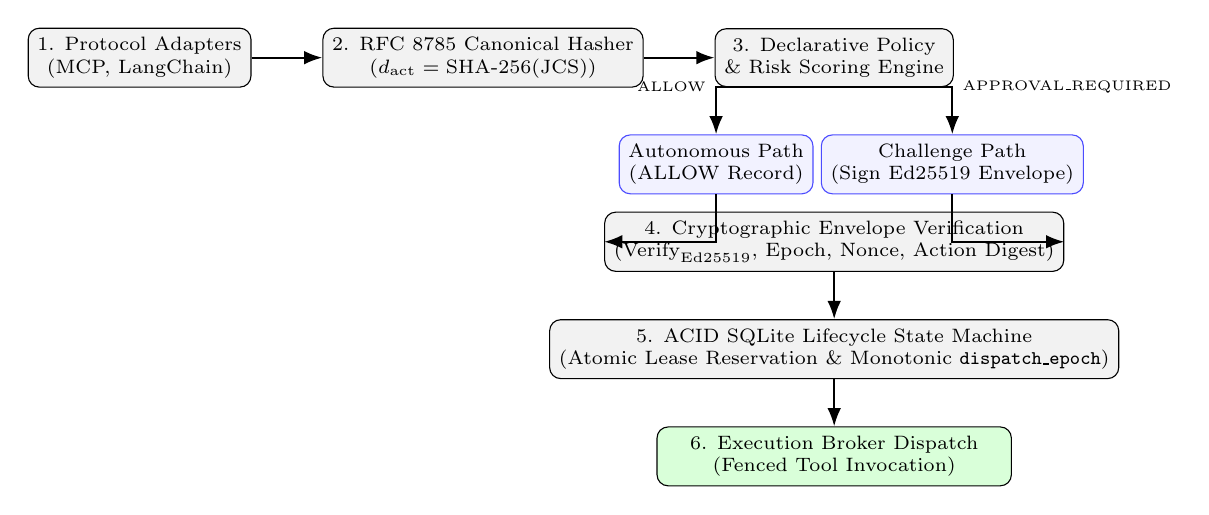
\begin{tikzpicture}[
    node distance=0.6cm and 0.9cm,
    stage/.style={rectangle, draw, rounded corners, minimum height=0.65cm, minimum width=2.4cm, align=center, fill=gray!10, font=\scriptsize},
    branch/.style={rectangle, draw=blue!70, rounded corners, minimum height=0.65cm, minimum width=2.2cm, align=center, fill=blue!5, font=\scriptsize},
    arrow/.style={-Latex, thick}
]

\node[stage] (adapter) {1. Protocol Adapters\\(MCP, LangChain)};
\node[stage, right=of adapter] (hasher) {2. RFC 8785 Canonical Hasher\\($d_{\text{act}} = \text{SHA-256}(\text{JCS})$)};
\node[stage, right=of hasher] (policy) {3. Declarative Policy\\\& Risk Scoring Engine};

\node[branch, below=0.6cm of policy, xshift=-1.5cm] (auto) {Autonomous Path\\(ALLOW Record)};
\node[branch, below=0.6cm of policy, xshift=1.5cm] (human) {Challenge Path\\(Sign Ed25519 Envelope)};

\node[stage, below=0.6cm of $(auto)!0.5!(human)$, minimum width=4.5cm] (crypto) {4. Cryptographic Envelope Verification\\($\text{Verify}_{\text{Ed25519}}$, Epoch, Nonce, Action Digest)};

\node[stage, below=0.6cm of crypto, minimum width=4.5cm] (fencing) {5. ACID SQLite Lifecycle State Machine\\(Atomic Lease Reservation \& Monotonic \texttt{dispatch\_epoch})};

\node[stage, below=0.6cm of fencing, minimum width=4.5cm, fill=green!15] (dispatch) {6. Execution Broker Dispatch\\(Fenced Tool Invocation)};

\draw[arrow] (adapter) -- (hasher);
\draw[arrow] (hasher) -- (policy);
\draw[arrow] (policy.south) -| node[left, font=\tiny] {ALLOW} (auto.north);
\draw[arrow] (policy.south) -| node[right, font=\tiny] {APPROVAL\_REQUIRED} (human.north);
\draw[arrow] (auto.south) |- (crypto.west);
\draw[arrow] (human.south) |- (crypto.east);
\draw[arrow] (crypto) -- (fencing);
\draw[arrow] (fencing) -- (dispatch);

\end{tikzpicture}
\caption{End-to-end authorization, verification, and fenced execution pipeline.}
\label{fig:pipeline}
\end{figure*}

AI Firewall is structured into four modular subsystems: Adapter Normalization, Policy \& Risk Engine, Cryptographic Envelope Verifier, and the Transactional Execution Broker (Figure~\ref{fig:pipeline}).

\subsection{Canonical Action Identity}
Tool invocations arriving from different frameworks represent identical actions with differing formatting. AI Firewall maps all incoming proposals into a canonical schema:
\begin{equation}
\text{ActionProposal} = \langle P, I, R, B \rangle
\end{equation}
where:
\begin{itemize}
    \item $P = \langle \text{user\_id}, \text{agent\_id}, \text{session\_id} \rangle$ represents the calling principal.
    \item $I = \langle \text{tool\_server\_id}, \text{tool\_name}, \text{operation\_type}, \text{canonical\_params} \rangle$ captures the exact operation.
    \item $R = \langle \text{resource\_uri}, \text{preconditions} \rangle$ defines the target and TOCTOU preconditions.
    \item $B = \langle \text{policy\_version}, \text{policy\_epoch}, \text{idempotency\_key}, \text{expires\_at\_utc} \rangle$ specifies authorization parameters.
\end{itemize}

Parameters are normalized using the RFC 8785 JSON Canonicalization Scheme (JCS)~\cite{rfc8785}: dictionary keys are lexicographically sorted by UTF-16 code units, whitespace is removed, and floating-point values are formatted deterministically. The canonical action digest is computed as:
\begin{equation}
d_{\text{act}} = \text{SHA-256}(\text{JCS}(\text{ActionProposal}))
\end{equation}

\subsection{Declarative Policy \& Risk Scoring}
When an action is proposed, the Policy Engine evaluates registered rules. The evaluated risk score $S \in [0.0, 100.0]$ is computed as:
\begin{equation}
S = \min\left(100.0, \, B_{\text{base}} + W_{\text{taint}} \cdot T + \sum_i W_{\text{param}, i} \cdot P_i\right)
\end{equation}
where $B_{\text{base}}$ is the base tool risk tier, $T \in \{0, 1\}$ indicates untrusted context taint, and $P_i$ represents sensitive parameter multipliers. Risk scores map to authorization tiers:
\begin{itemize}
    \item \textbf{LOW\_RISK ($S < 20.0$):} Autonomous \texttt{ALLOW}. Authorized solely by a gateway-signed \texttt{AuthorizationDecisionRecord}.
    \item \textbf{MEDIUM\_RISK ($20.0 \le S < 70.0$):} \texttt{APPROVAL\_REQUIRED} (Standard Human Confirmation).
    \item \textbf{HIGH\_RISK ($S \ge 70.0$):} \texttt{APPROVAL\_REQUIRED} (Hardware-bound MFA / Elevated Role).
    \item \textbf{POLICY\_DENIED:} Immediate fail-closed rejection.
\end{itemize}

\subsection{Exact-Action Approval Envelopes}
When human approval is required, the gateway generates a challenge payload containing $d_{\text{act}}$. The reviewer inspects the canonical action details and issues an approval envelope:
\begin{equation}
\text{Envelope} = \langle \text{approval\_id}, d_{\text{act}}, \text{claims}, \sigma_{\text{Ed25519}} \rangle
\end{equation}
The envelope claims embed:
\begin{equation}
\text{claims} = \langle \text{nonce}, \text{auth\_level}, \text{reviewer\_id}, \text{key\_id}, \text{pol\_ver}, \text{pol\_epoch}, t_{\text{issued}}, t_{\text{expires}} \rangle
\end{equation}
Before redemption, the gateway verifies that:
\begin{enumerate}
    \item $\text{Verify}_{\text{Ed25519}}(\sigma, \text{claims} \,\|\, d_{\text{act}}, K_{\text{pub}}) = \text{True}$.
    \item $d_{\text{act}} == \text{SHA-256}(\text{JCS}(\text{CurrentAction}))$.
    \item $\text{claims.pol\_epoch} == \text{Gateway.current\_epoch}$.
    \item $t_{\text{current}} \le t_{\text{expires}}$ and $K_{\text{pub}}$ is not revoked.
\end{enumerate}

\subsection{Transactional Lifecycle \& Worker Fencing}

\begin{figure}[t]
\centering
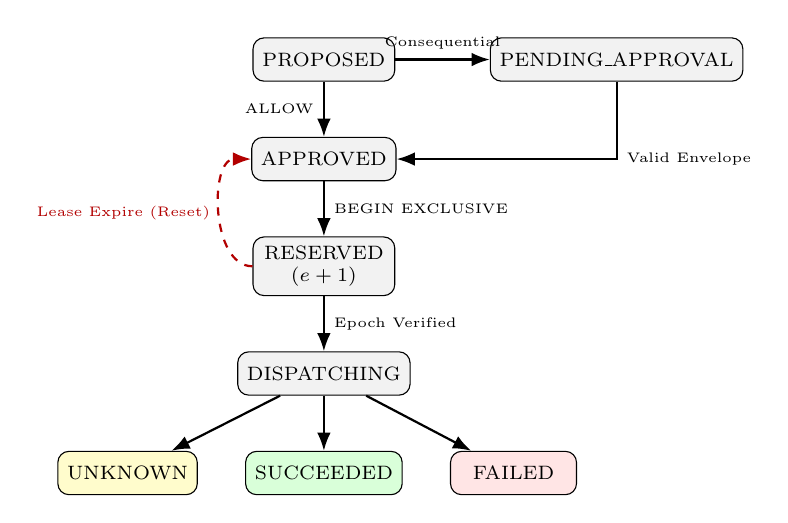
\begin{tikzpicture}[
    node distance=0.8cm and 0.8cm,
    state/.style={rectangle, draw, rounded corners, minimum height=0.55cm, minimum width=1.8cm, align=center, font=\scriptsize, fill=gray!10},
    term/.style={rectangle, draw, rounded corners, minimum height=0.55cm, minimum width=1.6cm, align=center, font=\scriptsize, fill=red!10},
    arrow/.style={-Latex, thick}
]
\node[state] (prop) {PROPOSED};
\node[state, right=1.2cm of prop] (pend) {PENDING\_APPROVAL};
\node[state, below=0.7cm of prop] (appr) {APPROVED};
\node[state, below=0.7cm of appr] (res) {RESERVED\\($e+1$)};
\node[state, below=0.7cm of res] (disp) {DISPATCHING};

\node[term, fill=green!15, below=0.7cm of disp] (succ) {SUCCEEDED};
\node[term, right=0.6cm of succ] (fail) {FAILED};
\node[term, fill=yellow!20, left=0.6cm of succ] (unk) {UNKNOWN};

\draw[arrow] (prop) -- node[above, font=\tiny] {Consequential} (pend);
\draw[arrow] (pend) |- node[right, font=\tiny] {Valid Envelope} (appr);
\draw[arrow] (prop) -- node[left, font=\tiny] {ALLOW} (appr);
\draw[arrow] (appr) -- node[right, font=\tiny] {BEGIN EXCLUSIVE} (res);
\draw[arrow] (res) -- node[right, font=\tiny] {Epoch Verified} (disp);

\draw[arrow] (disp) -- (succ);
\draw[arrow] (disp) -- (fail);
\draw[arrow] (disp) -- (unk);

\draw[arrow, dashed, red!70!black] (res.west) to[out=180,in=180] node[left, font=\tiny] {Lease Expire (Reset)} (appr.west);

\end{tikzpicture}
\caption{Lifecycle state machine and crash recovery boundaries.}
\label{fig:lifecycle}
\end{figure}

The gateway persists lifecycle state in SQLite with write-ahead logging (WAL). State transitions follow a strict directed graph (Figure~\ref{fig:lifecycle}). To prevent race conditions, reservation is executed inside \texttt{BEGIN EXCLUSIVE TRANSACTION}:
\begin{quote}
\small
\texttt{UPDATE approvals SET lifecycle\_state = 'RESERVED', worker\_id = ?, dispatch\_epoch = dispatch\_epoch + 1, lease\_expires\_at\_utc = ? WHERE approval\_id = ? AND lifecycle\_state = 'APPROVED';}
\end{quote}
If \texttt{rowcount != 1}, another worker won the race, and \texttt{ConcurrencyContentionError} is raised.

When transitioning to \texttt{DISPATCHING}, the gateway validates that the worker's token matches \texttt{(worker\_id, dispatch\_epoch)}. If a worker stalls and its lease expires, the background reaper recovers the lease:
\begin{itemize}
    \item If crashed in \texttt{RESERVED}: Reset to \texttt{APPROVED} (zero network bytes were sent; safe to re-reserve).
    \item If crashed in \texttt{DISPATCHING}: Transition to \texttt{UNKNOWN} (\texttt{ERR\_DISPATCH\_TIMEOUT\_UNKNOWN\_OUTCOME}). Automatic retries are strictly prohibited to prevent duplicate side effects.
\end{itemize}

%%
%% Section 5: Implementation
%%
\section{Implementation and Persistence Optimization}

The gateway is implemented in Python 3.14 with zero third-party framework dependencies outside standard cryptography (\texttt{pycryptodome}). 

\subsection{Analysis of Baseline Persistence Overhead}
During initial profiling in Phase 4.10, microbenchmarks of the un-optimized gateway revealed that pure canonicalization and policy computation accounted for only \textbf{1.28\%} of authorization latency (0.039\,ms), while SQLite persistence operations accounted for \textbf{98.72\%} (2.98\,ms). Profiling identified the root cause: each request opened and closed \textbf{8 separate database connections} across action recording, decision insertion, synthetic envelope generation, atomic reservation, dispatch transition, outcome update, and audit logging. Each connection executed two PRAGMA statements (\texttt{foreign\_keys = ON} and \texttt{journal\_mode = WAL}), causing repeated filesystem stat calls, lock acquisition, and WAL index header re-reads.

\subsection{Manager-Owned Thread Connection Registry}
To resolve this bottleneck without violating thread isolation or leaking operating system file descriptors upon manager shutdown, we replaced on-demand connection allocation with a \textbf{manager-owned thread connection registry}:
\begin{quote}
\small
\texttt{self.\_thread\_conns: dict[int, sqlite3.Connection] = \{\}}\\
\texttt{self.\_conns\_lock = threading.Lock()}
\end{quote}
When a worker thread requests a connection via \texttt{\_get\_connection()}:
\begin{enumerate}
    \item The manager acquires \texttt{\_conns\_lock} and inspects \texttt{\_thread\_conns} using the caller's integer thread identifier (\texttt{threading.get\_ident()}).
    \item If no connection exists, a dedicated connection is initialized with \texttt{check\_same\_thread=False} and cached in \texttt{\_thread\_conns}. PRAGMA statements are executed exactly once per thread.
    \item \textbf{Cross-Thread Shutdown Safety:} Because connections are initialized with \texttt{check\_same\_thread=False}, the managing orchestrator thread can safely iterate over \texttt{\_thread\_conns} during \texttt{close()} and invoke \texttt{.close()} on all connections without triggering \texttt{sqlite3.ProgrammingError}.
    \item \textbf{Post-Close Fail-Closed Behavior:} The manager sets an \texttt{\_is\_closed = True} sentinel. Subsequent calls to \texttt{\_get\_connection()} immediately raise \texttt{StorageError}, ensuring that workers cleanly abort during shutdown.
\end{enumerate}

Under this optimization, the persistence latency of an autonomous authorization drops from 2.98\,ms to $\sim$0.43\,ms. Pure computation (canonicalization, policy evaluation, and Ed25519 signing: $\sim$0.133\,ms) accounts for \textbf{23.6\%} of the pipeline, while transactional database persistence accounts for \textbf{76.4\%}.

%%
%% Section 6: Evaluation
%%
\section{Experimental Methodology and Results}

Our evaluation addresses five core research questions:

\subsection{RQ1 \& RQ2: Empirical Security Benchmark Evaluation (46 Scenarios)}
We evaluated AI Firewall against the established Phase 4.8.2 corrective benchmark comprising \textbf{46 discrete scenarios}: 31 consequential attack scenarios and 15 legitimate tasks. We compared System C (AI Firewall) against Baseline A (Direct Tool Execution without Mediation) and Baseline B (Policy Engine with Direct Dispatch).

\begin{table*}[t]
\centering
\caption{Comparative evaluation across the 46-scenario benchmark suite. Category 6 separates client schema failure (03A) from runtime broker authentication hierarchy rejection (03B).}
\label{tab:security_benchmark}
\small
\begin{tabular}{llll}
\toprule
\textbf{Scenario Category (Count)} & \textbf{Baseline A (Direct Execution)} & \textbf{Baseline B (Policy-Only)} & \textbf{System C (AI Firewall Ours)} \\
\midrule
Cat 1: Legitimate Read-Only (5)      & 5/5 Dispatched & 5/5 Dispatched & 5/5 Dispatched (\texttt{ALLOW}) \\
Cat 2: Legitimate Mutations (5)      & 5/5 Dispatched & 5/5 Dispatched & 5/5 Dispatched (\texttt{APPROVED}) \\
Cat 3: Direct Mandatory Denials (5)  & 5/5 Dispatched (Vulnerable) & 0/5 Dispatched (Blocked) & 0/5 Dispatched (\texttt{DENY}) \\
Cat 4: Untrusted Taint Elevation (5) & 5/5 Dispatched (Vulnerable) & 0/5 Dispatched (Blocked) & 0/5 Dispatched (\texttt{CHALLENGE}) \\
Cat 5: Privilege Escalation (5)      & 5/5 Dispatched (Vulnerable) & 0/5 Dispatched (Blocked) & 0/5 Dispatched (\texttt{DENY}) \\
Cat 6: Envelope Tampering (6)        & 6/6 Dispatched (Vulnerable) & 6/6 Dispatched (Vulnerable) & 0/6 Dispatched (\texttt{BLOCKED}) \\
\quad -- CORR\_CAT6\_03A (Schema Invalid) & 1/1 Dispatched (Vulnerable) & 1/1 Dispatched (Vulnerable) & 0/1 Dispatched (\texttt{SIGN\_FAIL}) \\
\quad -- CORR\_CAT6\_03B (Broker Downgrade) & 1/1 Dispatched (Vulnerable) & 1/1 Dispatched (Vulnerable) & 0/1 Dispatched (\texttt{BROKER\_DENY}) \\
Cat 7: Replay \& Revocation (5)     & 5/5 Dispatched (Vulnerable) & 5/5 Dispatched (Vulnerable) & 0/5 Dispatched (\texttt{BLOCKED}) \\
Cat 8: TOCTOU State Drift (5)        & 5/5 Dispatched (Vulnerable) & 5/5 Dispatched (Vulnerable) & 0/5 Dispatched (\texttt{ABORTED}) \\
Cat 9: Core Direct Proposal (5)      & 5/5 Dispatched & 5/5 Dispatched & 5/5 Dispatched (\texttt{ALLOW}) \\
\midrule
\textbf{Total Consequential Attacks (Cats 3--8)} & \textbf{31 Attacks} & \textbf{31 Attacks} & \textbf{31 Attacks} \\
\textbf{Attacks Blocked (Observed Success)}      & 0 / 31 (0.0\%) & 15 / 31 (48.4\%) & \textbf{31 / 31 (100.0\%)} \\
\textbf{Clopper--Pearson 95\% Confidence Interval} & [0.0\%, 11.2\%] & [30.2\%, 66.9\%] & \textbf{[88.8\%, 100.0\%]} \\
\textbf{Unauthorized Dispatches (Vulnerable)}    & 31 / 31 (100.0\%) & 16 / 31 (51.6\%) & \textbf{0 / 31 (0.0\%)} \\
\textbf{Legitimate Tasks Completed (Cats 1, 2, 9)} & 15 / 15 (100.0\%) & 15 / 15 (100.0\%) & \textbf{15 / 15 (100.0\%)} \\
\textbf{Clopper--Pearson 95\% Confidence Interval} & [78.2\%, 100.0\%] & [78.2\%, 100.0\%] & \textbf{[78.2\%, 100.0\%]} \\
\bottomrule
\end{tabular}
\end{table*}

\textbf{Empirical Findings (Table~\ref{tab:security_benchmark}):}
\begin{itemize}
    \item Baseline A suffered 100\% exploit success across all 31 attacks.
    \item Baseline B successfully blocked policy-denied tools (Cats 3--5) but was completely vulnerable (16/16 dispatches) to approval-bypass attacks, parameter tampering (Cat 6), approval replay (Cat 7), and TOCTOU precondition drift (Cat 8).
    \item System C successfully blocked all 31 consequential attacks (100.0\% observed, 95\% CI [88.8\%, 100.0\%]) while completing all 15 legitimate tasks without false denials (95\% CI [78.2\%, 100.0\%]). We note that this observed 100\% rate describes the evaluated synthetic scenario suite and does not establish a universal zero-failure probability against arbitrary real-world LLM attacks.
\end{itemize}

\subsection{Regression and Invariant Test Suite (107 Tests)}
In addition to the 46-scenario benchmark, the gateway's implementation is verified by a 107-test unit and regression suite executing in 0.55--0.61 seconds:
\begin{itemize}
    \item \textbf{Canonicalization \& Hasher (22 tests):} Deterministic JCS sorting, UTF-16 code units, number representations.
    \item \textbf{Cryptographic Envelopes \& Key Registry (18 tests):} Ed25519 signature checks, expiration timestamps, key revocation.
    \item \textbf{Policy Engine (15 tests):} Mandatory deny precedence, taint propagation, auth tier mapping.
    \item \textbf{SQLite Lifecycle \& Worker Fencing (10 tests):} Schema constraints, monotonic epochs, lease expiration.
    \item \textbf{Execution Broker \& Preconditions (10 tests):} Precondition hashing, challenge emission, broker dispatch gates.
    \item \textbf{Hardening \& Deduplication (12 tests):} Single-use nonces, parameter binding, replay prevention.
    \item \textbf{Adapter Mappings \& Parity (11 tests):} Schema conversion, error handling, cross-adapter parity.
    \item \textbf{MCP Stdio Subprocess (9 tests):} Real OS child-process pipes, JSON-RPC framing, downstream invocation tracing.
    \item \textbf{Simulated LangGraph Checkpoints (7 tests):} Interrupt cycles, dictionary state reload across restarts.
    \item \textbf{Connection Registry \& Concurrency (16 tests):} Deterministic cleanup, 8 crash-recovery scenarios, 20-thread concurrency.
\end{itemize}

\subsection{RQ3 \& RQ4: Performance Optimization and Scalability Benchmark}
We benchmarked the end-to-end Autonomous \texttt{ALLOW} pipeline (canonicalization + policy evaluation + Ed25519 signing + database transactions + dispatch + audit logging) on Linux x86\_64. We compared baseline on-demand connections against the thread-bounded connection registry over 100 timed trials (20 warmup runs) and a 200-operation throughput batch.

\begin{table}[t]
\centering
\caption{Microbenchmark performance comparison between on-demand and connection-registry configurations (calculated over 100 timed trials after 20 untimed warmup runs using $P_k = S[\lfloor n \cdot k \rfloor]$ on a zero-indexed array $S$).}
\label{tab:performance}
\small
\begin{tabular}{llll}
\toprule
\textbf{Metric} & \textbf{Baseline (On-Demand)} & \textbf{Optimized (Registry)} & \textbf{Delta / Improvement} \\
\midrule
Median Latency   & 3.0153\,ms  & 0.5643\,ms  & \textbf{-81.29\% (-2.451\,ms)} \\
P95 Latency      & 3.7991\,ms  & 0.8325\,ms  & \textbf{-78.09\% (-2.967\,ms)} \\
P99 Tail Latency & 24.0348\,ms & 0.9679\,ms  & \textbf{-95.97\% (-23.067\,ms)} \\
Mean Latency     & 3.0986\,ms  & 0.5909\,ms  & \textbf{-80.93\% (-2.508\,ms)} \\
Min Latency      & 2.0183\,ms  & 0.5180\,ms  & \textbf{-74.33\% (-1.500\,ms)} \\
Max Latency      & 24.0348\,ms & 0.9679\,ms  & \textbf{-95.97\% (-23.067\,ms)} \\
Batch Throughput & 397.7\,ops/s & 1,716.4\,ops/s & \textbf{+331.58\% (+1318.7)} \\
\bottomrule
\end{tabular}
\end{table}

Under connection caching (Table~\ref{tab:performance}), median latency dropped from \textbf{3.0153\,ms to 0.5643\,ms}, representing an \textbf{81.29\% reduction}. Most notably, tail latency (P99) fell by \textbf{95.97\%} (from 24.03\,ms down to 0.97\,ms), as connection caching eliminated intermittent lock contention and file-descriptor allocation stalls.

\begin{table}[t]
\centering
\caption{Multithreaded and multiprocess scaling under the connection registry.}
\label{tab:concurrency}
\small
\begin{tabular}{lllll}
\toprule
\textbf{Configuration} & \textbf{Concurrency} & \textbf{Total Ops} & \textbf{Median Latency} & \textbf{Throughput} \\
\midrule
Multithreaded & 10 Threads  & 300 Ops & 0.7075\,ms & 1,167.1\,ops/sec \\
Multiprocess  & 4 Processes & 200 Ops & 0.6165\,ms & 1,265.9\,ops/sec \\
\bottomrule
\end{tabular}
\end{table}

Under concurrent write loads (Table~\ref{tab:concurrency}), median latency remained sub-millisecond (0.71\,ms and 0.62\,ms). P95/P99 latencies exhibited expected increases (34.31\,ms and 5.99\,ms) due to SQLite's serialized \texttt{BEGIN EXCLUSIVE TRANSACTION} locking, confirming safe serial execution without lock corruption.

\subsection{RQ5: Integration Validation \& Cross-Adapter Parity}
We verified protocol interoperability across two adapter paradigms:
\begin{enumerate}
    \item \textbf{Model Context Protocol (MCP):} Evaluated by executing an actual OS child process running \texttt{MCPAdapter} over standard input/output pipes with JSON-RPC 2.0 framing. All 9 test cases passed, verifying protocol challenge interception and fenced execution over real OS pipes.
    \item \textbf{LangChain / LangGraph:} Evaluated across 7 test cases simulating graph interrupt and state checkpoint serialization across simulated process restarts.
    \item \textbf{Cross-Adapter Parity:} 5 paired test cases demonstrated that identical user tool invocations originating from either MCP or LangChain produced identical canonical hashes ($d_{\text{act}}$) and identical policy verdicts.
\end{enumerate}

%%
%% Section 7: Discussion
%%
\section{Discussion and Security Analysis}

\subsection{Defense-in-Depth vs. Model Alignment}
A recurring theme in recent AI safety research is that LLM prompt alignment is fundamentally non-robust~\cite{greshake2023not, debenedetti2024agentdojo}. Adversaries continuously discover jailbreaks, multi-lingual encodings, and prompt-injection perturbations that bypass system prompts. AI Firewall treats the entire LLM reasoning pipeline as untrusted, enforcing security invariants at the deterministic network boundary. Even if an agent's internal reasoning is compromised, it cannot produce valid cryptographic signatures over unauthorized canonical digests.

\subsection{The Wire Dispatch Boundary \& Downstream Idempotency}
A crucial security boundary identified in our audit involves post-dispatch crashes. When the gateway transitions an approval to \texttt{DISPATCHING} and sends bytes over the network wire, it cannot revoke those packets if the worker process crashes before recording the result:
\begin{equation}
\text{Gateway Fencing} \neq \text{End-to-End Exactly-Once}
\end{equation}
While the gateway marks the internal state as \texttt{UNKNOWN} and prohibits automatic re-dispatch, duplicate side effects can occur if the downstream tool endpoint is not idempotent. Therefore, we formalize the requirement that downstream services executing consequential actions must accept an \texttt{Idempotency-Key} or enforce conditional request fencing based on $d_{\text{act}}$.

%%
%% Section 8: Limitations
%%
\section{Limitations and Threats to Validity}
\begin{enumerate}
    \item \textbf{Synthetic Evaluation Suite:} While our 46-scenario benchmark and 107 regression tests cover adversarial parameter mutations, timing races, and protocol errors, they represent a curated synthetic test suite rather than a live multi-tenant production deployment.
    \item \textbf{Third-Party Package Absences:} The official \texttt{mcp} and \texttt{langgraph} pip packages were not installed in the test environment. While protocol framing was validated via real OS subprocess stdio pipes, testing with official SDK runtime classes remains future work.
    \item \textbf{Transport Scope:} Integration was evaluated over local stdio and in-process interfaces; remote MCP transports (HTTP Server-Sent Events) and distributed database backends (PostgreSQL) were not benchmarked.
    \item \textbf{Human Reviewer Trust:} The security of the human-in-the-loop mechanism assumes that the human reviewer carefully inspects canonicalized parameters rather than blindly signing approval challenges.
\end{enumerate}

%%
%% Section 9: Reproducibility
%%
\section{Reproducibility}
To ensure complete scientific reproducibility, all source code, tests, and raw measurement data are archived in the repository:
\begin{itemize}
    \item \textbf{Core Implementation:} \texttt{src/ai\_firewall/}
    \item \textbf{Regression Suite (107 Tests):}\ \texttt{pytest -o pythonpath=src -q} (execution time: 0.55\,s)
    \item \textbf{Corrective Benchmark Suite (46 Scenarios):}\ \texttt{scratch/corrective\_benchmark\_harness.py}
    \item \textbf{Real MCP Subprocess Harness:}\ \texttt{tests/test\_mcp\_subprocess\_integration.py}
    \item \textbf{Crash Recovery \& Concurrency Suite:}\ \texttt{tests/test\_connection\_lifecycle\_and\_recovery.py}
    \item \textbf{Frozen Benchmark Vectors:}\ \texttt{phase\_4\_11\_raw\_benchmark\_results.json} and \texttt{phase\_4\_12\_raw\_verification\_results.json}
\end{itemize}

%%
%% Section 10: Conclusion
%%
\section{Conclusion and Future Work}
We presented \textbf{AI Firewall}, a shared, risk-based authorization gateway for autonomous AI agents. By coupling RFC 8785 canonical action identity with Ed25519 cryptographic approval envelopes, AI Firewall eliminates parameter tampering, approval substitution, and replay attacks across heterogeneous agent adapters. ACID-compliant SQLite lifecycle management with monotonic dispatch epoch fencing guarantees safe mutual exclusion and fail-closed crash recovery. Through a manager-owned thread connection registry, the gateway achieves sub-millisecond median latency (0.56\,ms) and 1,716\,ops/sec throughput, demonstrating that rigorous runtime authorization imposes negligible overhead on AI agent execution.

Future work will focus on integrating enterprise Key Management Systems (KMS), benchmarking remote HTTP/SSE MCP transports, and validating official SDK runtimes across live multi-agent production deployments.

%%
%% Bibliography
%%
\bibliographystyle{ACM-Reference-Format}
\bibliography{references}

\end{document}

